\documentclass{standalone}
\usepackage{tikz}
\usetikzlibrary{patterns, positioning}


\begin{document}
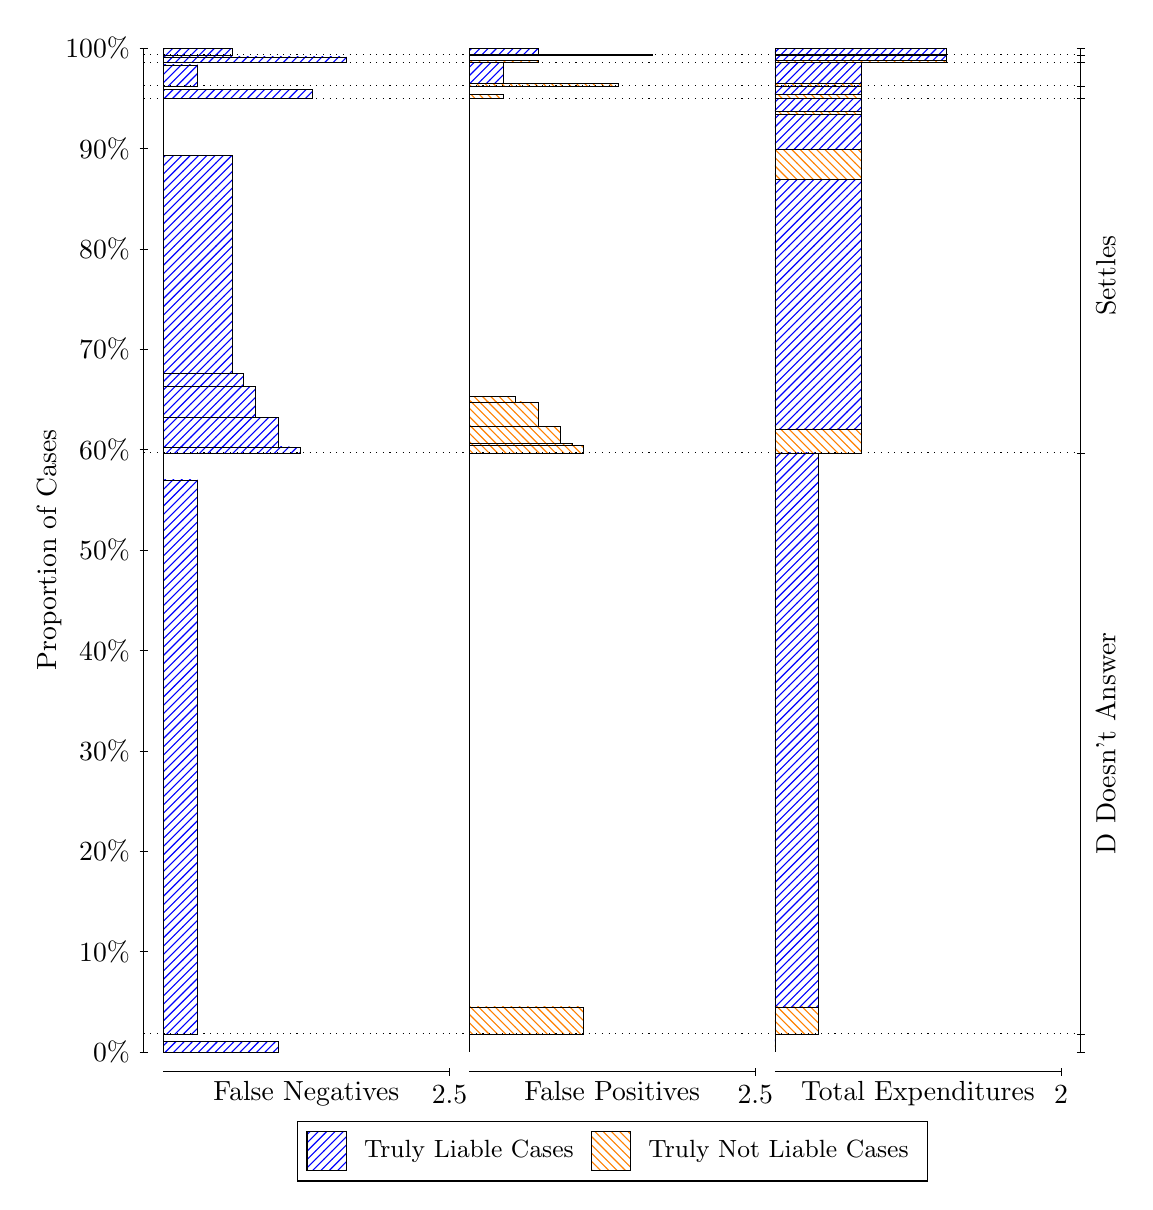
\begin{tikzpicture}
\draw[black, very thin] (1.5,1.75) -- (1.5,14.5);
\node[rotate=90, text=black, anchor=center] at (0.3, 8.125) {Proportion of Cases};
\draw[black, very thin] (1.45,1.75) -- (1.55,1.75);
\node[text=black, anchor=east] at (1.45, 1.75) {0\%};
\draw[black, very thin] (1.45,3.025) -- (1.55,3.025);
\node[text=black, anchor=east] at (1.45, 3.025) {10\%};
\draw[black, very thin] (1.45,4.3) -- (1.55,4.3);
\node[text=black, anchor=east] at (1.45, 4.3) {20\%};
\draw[black, very thin] (1.45,5.575) -- (1.55,5.575);
\node[text=black, anchor=east] at (1.45, 5.575) {30\%};
\draw[black, very thin] (1.45,6.85) -- (1.55,6.85);
\node[text=black, anchor=east] at (1.45, 6.85) {40\%};
\draw[black, very thin] (1.45,8.125) -- (1.55,8.125);
\node[text=black, anchor=east] at (1.45, 8.125) {50\%};
\draw[black, very thin] (1.45,9.4) -- (1.55,9.4);
\node[text=black, anchor=east] at (1.45, 9.4) {60\%};
\draw[black, very thin] (1.45,10.675) -- (1.55,10.675);
\node[text=black, anchor=east] at (1.45, 10.675) {70\%};
\draw[black, very thin] (1.45,11.95) -- (1.55,11.95);
\node[text=black, anchor=east] at (1.45, 11.95) {80\%};
\draw[black, very thin] (1.45,13.225) -- (1.55,13.225);
\node[text=black, anchor=east] at (1.45, 13.225) {90\%};
\draw[black, very thin] (1.45,14.5) -- (1.55,14.5);
\node[text=black, anchor=east] at (1.45, 14.5) {100\%};

\draw[black, very thin] (13.4,1.75) -- (13.4,14.5);
\draw[black, very thin] (13.35,1.75) -- (13.45,1.75);
\node[anchor=west] at (13.35, 1.75) {};
\draw[black, very thin] (13.35,1.9792) -- (13.45,1.9792);
\node[anchor=west] at (13.35, 1.9792) {};
\draw[black, very thin] (13.35,9.3584) -- (13.45,9.3584);
\node[anchor=west] at (13.35, 9.3584) {};
\draw[black, very thin] (13.35,13.857) -- (13.45,13.857);
\node[anchor=west] at (13.35, 13.857) {};
\draw[black, very thin] (13.35,14.02) -- (13.45,14.02);
\node[anchor=west] at (13.35, 14.02) {};
\draw[black, very thin] (13.35,14.32) -- (13.45,14.32);
\node[anchor=west] at (13.35, 14.32) {};
\draw[black, very thin] (13.35,14.414) -- (13.45,14.414);
\node[anchor=west] at (13.35, 14.414) {};
\draw[black, very thin] (13.35,14.5) -- (13.45,14.5);
\node[anchor=west] at (13.35, 14.5) {};

\draw[black, very thin, pattern color=blue, pattern=north east lines] (1.75,1.75) rectangle (3.2033,1.8796);
\draw[black, very thin, pattern color=orange, pattern=north west lines] (1.75,1.8796) rectangle (1.75,1.9792);
\draw[black, very thin, pattern color=blue, pattern=north east lines] (1.75,1.9792) rectangle (2.186,9.0161);
\draw[black, very thin, pattern color=orange, pattern=north west lines] (1.75,9.0161) rectangle (1.75,9.3584);
\draw[black, very thin, pattern color=blue, pattern=north east lines] (1.75,9.3584) rectangle (3.494,9.4305);
\draw[black, very thin, pattern color=blue, pattern=north east lines] (1.75,9.4305) rectangle (3.3487,9.4351);
\draw[black, very thin, pattern color=blue, pattern=north east lines] (1.75,9.4351) rectangle (3.2033,9.8099);
\draw[black, very thin, pattern color=blue, pattern=north east lines] (1.75,9.8099) rectangle (2.9127,10.204);
\draw[black, very thin, pattern color=blue, pattern=north east lines] (1.75,10.204) rectangle (2.7673,10.37);
\draw[black, very thin, pattern color=blue, pattern=north east lines] (1.75,10.37) rectangle (2.622,13.141);
\draw[black, very thin, pattern color=orange, pattern=north west lines] (1.75,13.141) rectangle (1.75,13.857);
\draw[black, very thin, pattern color=blue, pattern=north east lines] (1.75,13.857) rectangle (3.6393,13.97);
\draw[black, very thin, pattern color=orange, pattern=north west lines] (1.75,13.97) rectangle (1.75,14.02);
\draw[black, very thin, pattern color=blue, pattern=north east lines] (1.75,14.02) rectangle (2.186,14.286);
\draw[black, very thin, pattern color=orange, pattern=north west lines] (1.75,14.286) rectangle (1.75,14.32);
\draw[black, very thin, pattern color=blue, pattern=north east lines] (1.75,14.32) rectangle (4.0753,14.388);
\draw[black, very thin, pattern color=orange, pattern=north west lines] (1.75,14.388) rectangle (1.75,14.414);
\draw[black, very thin, pattern color=blue, pattern=north east lines] (1.75,14.414) rectangle (2.622,14.493);
\draw[black, very thin, pattern color=orange, pattern=north west lines] (1.75,14.493) rectangle (1.75,14.5);
\draw[black, very thin, pattern color=orange, pattern=north west lines] (5.6333,1.75) rectangle (5.6333,1.8496);
\draw[black, very thin, pattern color=blue, pattern=north east lines] (5.6333,1.8496) rectangle (5.6333,1.9792);
\draw[black, very thin, pattern color=orange, pattern=north west lines] (5.6333,1.9792) rectangle (7.0867,2.3215);
\draw[black, very thin, pattern color=blue, pattern=north east lines] (5.6333,2.3215) rectangle (5.6333,9.3584);
\draw[black, very thin, pattern color=orange, pattern=north west lines] (5.6333,9.3584) rectangle (7.0867,9.453);
\draw[black, very thin, pattern color=orange, pattern=north west lines] (5.6333,9.453) rectangle (6.9413,9.4824);
\draw[black, very thin, pattern color=orange, pattern=north west lines] (5.6333,9.4824) rectangle (6.796,9.6921);
\draw[black, very thin, pattern color=orange, pattern=north west lines] (5.6333,9.6921) rectangle (6.5053,10.004);
\draw[black, very thin, pattern color=orange, pattern=north west lines] (5.6333,10.004) rectangle (6.36,10.007);
\draw[black, very thin, pattern color=orange, pattern=north west lines] (5.6333,10.007) rectangle (6.2147,10.074);
\draw[black, very thin, pattern color=blue, pattern=north east lines] (5.6333,10.074) rectangle (5.6333,13.857);
\draw[black, very thin, pattern color=orange, pattern=north west lines] (5.6333,13.857) rectangle (6.0693,13.907);
\draw[black, very thin, pattern color=blue, pattern=north east lines] (5.6333,13.907) rectangle (5.6333,14.02);
\draw[black, very thin, pattern color=orange, pattern=north west lines] (5.6333,14.02) rectangle (7.5227,14.054);
\draw[black, very thin, pattern color=blue, pattern=north east lines] (5.6333,14.054) rectangle (6.0693,14.32);
\draw[black, very thin, pattern color=orange, pattern=north west lines] (5.6333,14.32) rectangle (6.5053,14.346);
\draw[black, very thin, pattern color=blue, pattern=north east lines] (5.6333,14.346) rectangle (5.6333,14.414);
\draw[black, very thin, pattern color=orange, pattern=north west lines] (5.6333,14.414) rectangle (7.9587,14.421);
\draw[black, very thin, pattern color=blue, pattern=north east lines] (5.6333,14.421) rectangle (6.5053,14.5);
\draw[black, very thin, pattern color=orange, pattern=north west lines] (9.5167,1.75) rectangle (9.5167,1.8496);
\draw[black, very thin, pattern color=blue, pattern=north east lines] (9.5167,1.8496) rectangle (9.5167,1.9792);
\draw[black, very thin, pattern color=orange, pattern=north west lines] (9.5167,1.9792) rectangle (10.062,2.3215);
\draw[black, very thin, pattern color=blue, pattern=north east lines] (9.5167,2.3215) rectangle (10.062,9.3584);
\draw[black, very thin, pattern color=orange, pattern=north west lines] (9.5167,9.3584) rectangle (10.607,9.6627);
\draw[black, very thin, pattern color=blue, pattern=north east lines] (9.5167,9.6627) rectangle (10.607,12.828);
\draw[black, very thin, pattern color=orange, pattern=north west lines] (9.5167,12.828) rectangle (10.607,13.21);
\draw[black, very thin, pattern color=blue, pattern=north east lines] (9.5167,13.21) rectangle (10.607,13.662);
\draw[black, very thin, pattern color=orange, pattern=north west lines] (9.5167,13.662) rectangle (10.607,13.691);
\draw[black, very thin, pattern color=blue, pattern=north east lines] (9.5167,13.691) rectangle (10.607,13.857);
\draw[black, very thin, pattern color=orange, pattern=north west lines] (9.5167,13.857) rectangle (10.607,13.907);
\draw[black, very thin, pattern color=blue, pattern=north east lines] (9.5167,13.907) rectangle (10.607,14.02);
\draw[black, very thin, pattern color=orange, pattern=north west lines] (9.5167,14.02) rectangle (10.607,14.054);
\draw[black, very thin, pattern color=blue, pattern=north east lines] (9.5167,14.054) rectangle (10.607,14.32);
\draw[black, very thin, pattern color=orange, pattern=north west lines] (9.5167,14.32) rectangle (11.697,14.346);
\draw[black, very thin, pattern color=blue, pattern=north east lines] (9.5167,14.346) rectangle (11.697,14.414);
\draw[black, very thin, pattern color=orange, pattern=north west lines] (9.5167,14.414) rectangle (11.697,14.421);
\draw[black, very thin, pattern color=blue, pattern=north east lines] (9.5167,14.421) rectangle (11.697,14.5);
\draw[black, dotted] (1.5,1.9792) -- (13.4,1.9792);
\draw[black, dotted] (1.5,9.3584) -- (13.4,9.3584);
\draw[black, dotted] (1.5,13.857) -- (13.4,13.857);
\draw[black, dotted] (1.5,14.02) -- (13.4,14.02);
\draw[black, dotted] (1.5,14.32) -- (13.4,14.32);
\draw[black, dotted] (1.5,14.414) -- (13.4,14.414);
\draw[black, very thin] (1.75,1.5) -- (5.3833,1.5);
\node[text=black, anchor=north] at (3.5667, 1.5) {False Negatives};
\draw[black, very thin] (5.3833,1.45) -- (5.3833,1.55);
\node[text=black, anchor=north] at (5.3833, 1.45) {2.5};

\draw[black, very thin] (5.6333,1.5) -- (9.2667,1.5);
\node[text=black, anchor=north] at (7.45, 1.5) {False Positives};
\draw[black, very thin] (9.2667,1.45) -- (9.2667,1.55);
\node[text=black, anchor=north] at (9.2667, 1.45) {2.5};

\draw[black, very thin] (9.5167,1.5) -- (13.15,1.5);
\node[text=black, anchor=north] at (11.333, 1.5) {Total Expenditures};
\draw[black, very thin] (13.15,1.45) -- (13.15,1.55);
\node[text=black, anchor=north] at (13.15, 1.45) {2};


\node[text=black, centered, rotate=90] at (13.72, 5.6688) {D Doesn't Answer};
\node[text=black, centered, rotate=90] at (13.72, 11.608) {Settles};





\draw (7.449999999999999,1.5) node[draw=none] (baseCoordinate) {};
\begin{scope}[align=center]
        \matrix[scale=0.5, draw=black, below=0.5cm of baseCoordinate, nodes={draw}, column sep=0.1cm]{
            \node[rectangle, draw, minimum width=0.5cm, minimum height=0.5cm, pattern color=blue, pattern=north east lines] {}; &
            \node[draw=none, font=\small, text=black] (B) {Truly Liable Cases}; &
            \node[rectangle, draw, minimum width=0.5cm, minimum height=0.5cm, pattern color=orange, pattern=north west lines] {}; &
            \node[draw=none, font=\small, text=black] (B) {Truly Not Liable Cases}; \\
            };
\end{scope}

\end{tikzpicture}
\end{document}